\documentclass[a4paper,12pt]{article}
%---------------------------------------------------------------
% Packages
%---------------------------------------------------------------

\usepackage[utf8]{inputenc}
\usepackage[english]{babel}
\usepackage{amsmath}          % For advanced math typesetting
\usepackage{amssymb}          % For math symbols
\usepackage{graphicx}         % To include images
\usepackage[margin=1in]{geometry} % For setting page margins
\usepackage{hyperref}         % For creating hyperlinks
\usepackage{listings}         % For code listings
\usepackage{xcolor}           % For defining colors
\usepackage{fancyhdr}         % For custom headers and footers
\usepackage{booktabs}         % For better looking tables
\usepackage{float}            % For figure placement
\usepackage{subcaption}       % For sub-figures

%---------------------------------------------------------------
% Hyperlink Setup
%---------------------------------------------------------------

\hypersetup{
    colorlinks=true,
    linkcolor=blue,
    filecolor=magenta,      
    urlcolor=cyan,
    pdftitle={Lab Report},
    pdfpagemode=FullScreen,
}

%---------------------------------------------------------------
% Code Listing Style
%---------------------------------------------------------------

\definecolor{codegreen}{rgb}{0,0.6,0}
\definecolor{codegray}{rgb}{0.5,0.5,0.5}
\definecolor{codepurple}{rgb}{0.58,0,0.82}
\definecolor{backcolour}{rgb}{0.95,0.95,0.95}

\lstdefinestyle{mystyle}{
    backgroundcolor=\color{backcolour},   
    commentstyle=\color{codegreen},
    keywordstyle=\color{magenta},
    numberstyle=\tiny\color{codegray},
    stringstyle=\color{codepurple},
    basicstyle=\ttfamily\footnotesize,
    breakatwhitespace=false,         
    breaklines=true,                 
    captionpos=b,                    
    keepspaces=true,                 
    numbers=left,                    
    numbersep=5pt,                  
    showspaces=false,                
    showstringspaces=false,
    showtabs=false,                  
    tabsize=2
}
\lstset{style=mystyle}

%---------------------------------------------------------------
% Header and Footer
%---------------------------------------------------------------

\setlength{\headheight}{15pt} % 增加页眉高度以容纳内容
\pagestyle{fancy}
\fancyhf{} % clear all header and footer fields
\fancyhead[L]{ADS Project VII - Skip List}
\fancyfoot[C]{\thepage}
\renewcommand{\headrulewidth}{0.4pt}
\renewcommand{\footrulewidth}{0.4pt}

%---------------------------------------------------------------
% Title Information
%---------------------------------------------------------------

\title{
    \centering
    \vspace{1cm}
    %顶部图片
    
\includegraphics[width=0.35\paperwidth]{images/cover.png}\par
    \vspace{2cm}
    %标题
    {\Huge\bfseries Project VII:\\[0.5em]Skip List\par}
    \vspace{0.5cm}
    {Advanced Data Structures and Algorithms Analysis}\par
    \vspace{1cm}
}
\author{
    \textbf{Group1: Lin Zhiyu, Hu Junyu, Huang Zhenhua} \\[0.5cm]
    \textit{College of Computer Science and Technology} \\
    \textit{Zhejiang University}
}
\date{\today}

%---------------------------------------------------------------
% Document Body
%---------------------------------------------------------------

\begin{document}

\maketitle
\thispagestyle{empty} % No header/footer on the title page
\newpage

\newpage
\tableofcontents
\newpage

\section{Introduction}
The Skip List is a probabilistic data structure that serves as an alternative to balanced trees. It supports efficient searching, insertion, and deletion operations with an expected time complexity of $O(\log N)$. Unlike balanced trees (e.g., AVL or Red-Black trees), which require complex rebalancing operations to maintain their structure, Skip Lists rely on randomization to achieve balance, making them simpler to implement and often faster in practice due to better cache locality and lower constant factors.

In this project, we aim to implement a Skip List in C and rigorously analyze its performance. We will demonstrate that its operations indeed follow the $O(\log N)$ time complexity through extensive empirical testing. By varying the input size $N$ and measuring the execution time for insertion, deletion, and search operations, we will provide experimental evidence supporting the theoretical bounds.


\section{Algorithm Specification}

\subsection{Data Structures}
A Skip List is built upon multiple layers of linked lists.

The bottom layer (Level 0) is a standard sorted linked list containing all the elements. Each higher layer acts as an "express lane" for the lists below, containing a subset of the elements from the layer immediately below it. An element at layer $i$ appears in layer $i+1$ with a fixed probability $p$. This probabilistic promotion of elements creates a hierarchy of linked lists, allowing for faster traversal during search operations.

\begin{figure}[H]
    \centering
    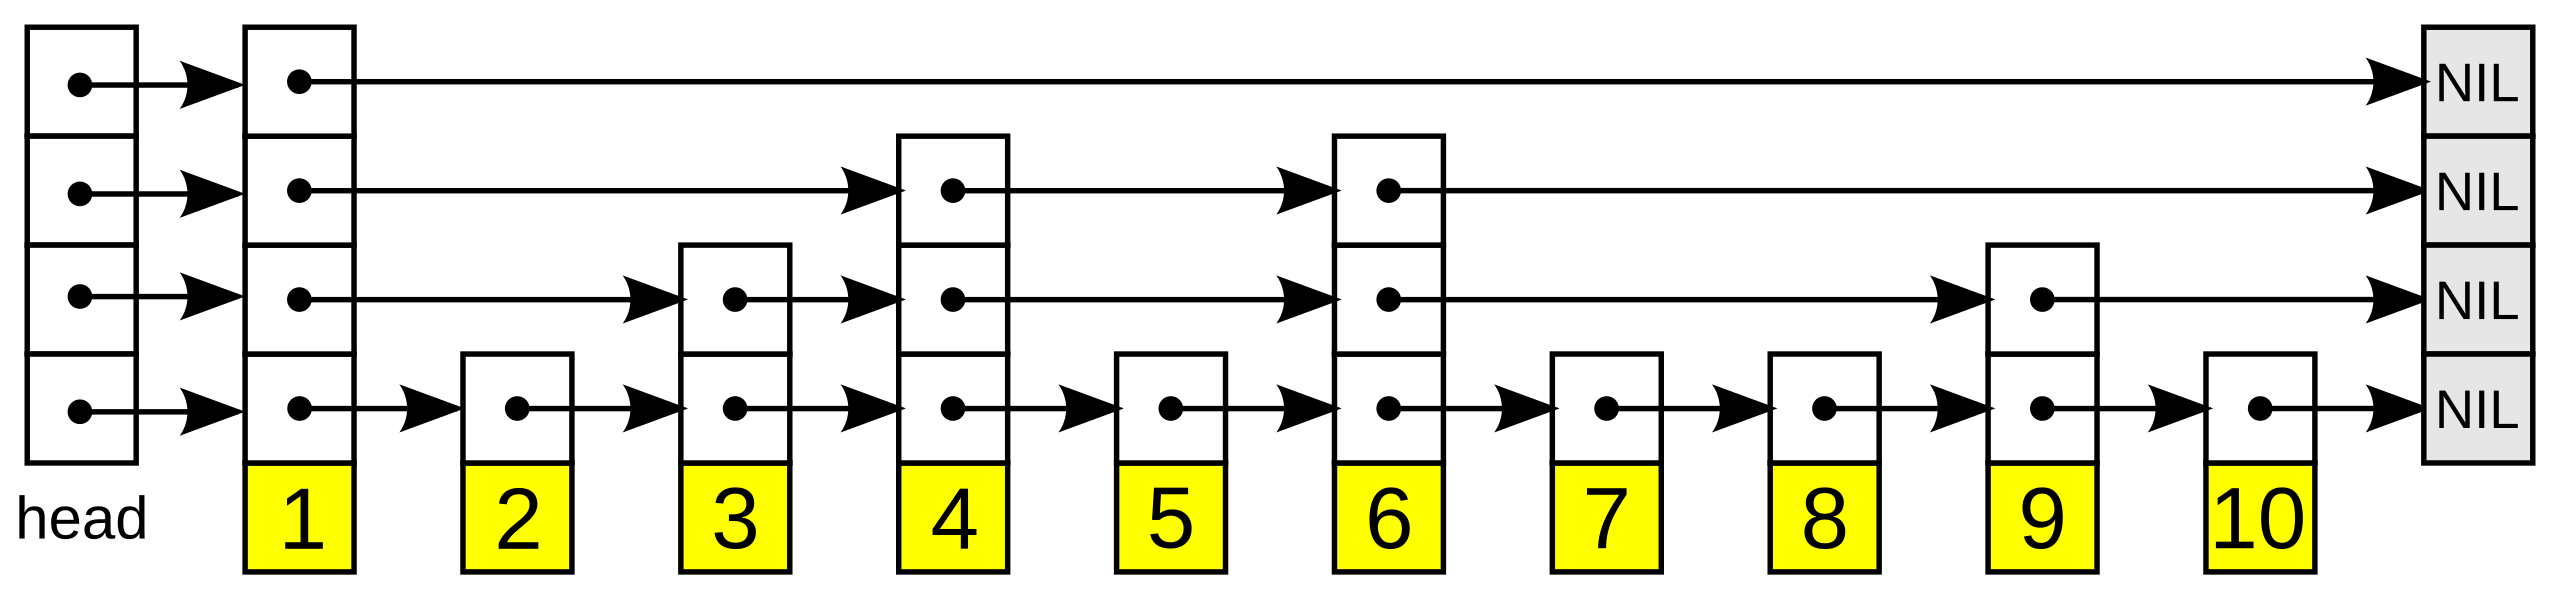
\includegraphics[width=0.9\textwidth]{images/Skip_list.png}
    \caption{A schematic picture of the skip list data structure. Each box with an arrow represents a pointer and a row is a linked list giving a sparse subsequence; the numbered boxes (in yellow) at the bottom represent the ordered data sequence. Searching proceeds downwards from the sparsest subsequence at the top until consecutive elements bracketing the search element are found.}
    \label{fig:skiplist_structure}
\end{figure}

In our implementation, we define the node structure as follows:

\begin{lstlisting}[language=C]
typedef struct skip_list_node {
    int data; // the value of the node
    int maxLevel; // the level of the node
    struct skip_list_node *forward[MAX_LEVEL]; // the next node pointers for each level
} skip_list_node;

typedef struct skip_list {
    int levelCount; // the  highest level of the skip list
    skip_list_node *head; // pointer to the head node of the skip list
} skip_list;
\end{lstlisting}

\begin{itemize}
    \item \textbf{data}: The integer value stored in the node.
    \item \textbf{maxLevel}: The maximum level of the node, determined at creation time.
    \item \textbf{forward}: An array of pointers. `forward[i]` points to the next node in the $i$-th level. The size of this array is fixed to \texttt{MAX\_LEVEL} (24) in our implementation to simplify memory management.
\end{itemize}

The skip list structure itself maintains:
\begin{itemize}
    \item \textbf{levelCount}: The current highest level of any node in the skip list.
    \item \textbf{head}: A pointer to the sentinel head node.
\end{itemize}

The head node is a sentinel node that does not store any actual data (initialized to -1). It serves as the starting point for all searches and is used to simplify the insertion and deletion algorithms by providing a valid node to point to at all times.

\subsection{Skip List Operations}
The main operations for the skip list are:

\subsubsection{Search}
To search for a value:
\begin{itemize}
    \item Start at the topmost layer of the head node.
    \item Move forward in the current layer until the next node's value is greater than or equal to the target value, or until the end of the layer.
    \item If the next node's value is less than the target, move to that node.
    \item If the next node's value is greater or equal (or NULL), descend to the next lower layer.
    \item Repeat until the bottom layer is reached.
    \item Check if the node at the bottom layer contains the target value.
\end{itemize}

\begin{lstlisting}[language=C]
function search(list, value):
    p = list->head
    for i from list->levelCount - 1 down to 0:
        while p->forward[i] is not NULL and p->forward[i]->data < value:
            p = p->forward[i]
    
    if p->forward[0] is not NULL and p->forward[0]->data == value:
        return p->forward[0]
    else:
        return NULL
\end{lstlisting}

\subsubsection{Insertion}
To insert a value:
\begin{itemize}
    \item Locate the position for the new value by traversing from the top level down, similar to the search operation.
    \item Keep track of the "update" path: an array of pointers to the nodes that will precede the new node at each level.
    \item If the value already exists, return (no duplicates).
    \item Generate a random level for the new node.
    \item If the new level is higher than the current list level, update the list level and initialize the update array for the new levels to point to the head.
    \item Create the new node and insert it into the linked lists at each level up to its random level, updating the pointers using the "update" array.
\end{itemize}

\begin{lstlisting}[language=C]
function insert(list, value):
    update = array of size MAX_LEVEL
    p = list->head

    for i from list->levelCount - 1 down to 0:
        while p->forward[i] is not NULL and p->forward[i]->data < value:
            p = p->forward[i]
        update[i] = p
    
    if p->forward[0] is not NULL and p->forward[0]->data == value:
        return // Value already exists
    
    level = random_level()
    if level > list->levelCount:
        for i from list->levelCount to level - 1:
            update[i] = list->head
        list->levelCount = level
    
    newNode = create_node(value, level)
    for i from 0 to level - 1:
        newNode->forward[i] = update[i]->forward[i]
        update[i]->forward[i] = newNode
\end{lstlisting}

\subsubsection{Deletion}
To delete a value:
\begin{itemize}
    \item Locate the node to be deleted by traversing from the top level down, recording the "update" path (predecessors at each level).
    \item If the node is found at the bottom level:
    \begin{itemize}
        \item Remove the node from each level where it exists by updating the predecessors' pointers.
        \item Free the memory of the deleted node.
        \item If the deletion leaves the highest levels empty (pointing to NULL), decrease the list's level count.
    \end{itemize}
\end{itemize}

\begin{lstlisting}[language=C]
function delete(list, value):
    update = array of size MAX_LEVEL
    p = list->head

    for i from list->levelCount - 1 down to 0:
        while p->forward[i] is not NULL and p->forward[i]->data < value:
            p = p->forward[i]
        update[i] = p
    
    if p->forward[0] is not NULL and p->forward[0]->data == value:
        toDelete = p->forward[0]
        for i from list->levelCount - 1 down to 0:
            if update[i]->forward[i] is not NULL and update[i]->forward[i]->data == value:
                update[i]->forward[i] = update[i]->forward[i]->forward[i]
        
        free(toDelete)
        
        while list->levelCount > 1 and list->head->forward[list->levelCount - 1] is NULL:
            list->levelCount = list->levelCount - 1
\end{lstlisting}

\subsection{Skip List Construction}
The skip list is constructed by initializing a head node and setting the level count to 1.

\begin{lstlisting}[language=C]
function create_skip_list():
    list = allocate memory for skip_list
    list->levelCount = 1
    list->head = allocate memory for skip_list_node
    list->head->data = -1 // Sentinel value
    list->head->maxLevel = 0
    initialize list->head->forward with NULLs
    return list
\end{lstlisting}

\section{Theoretical Analysis}
In this section, we provide a formal proof that the expected time complexity for skip list operations is $O(\log N)$.

\subsection{Expected Time Complexity of Search}
We analyze the search path backwards, moving from the target node at the bottom level up to the head node at the top level. This process can be divided into two parts: climbing from level 0 to level $L(n)$, and the subsequent operations at the top levels.

Let $C(i)$ be the expected cost (number of steps) to climb $i$ levels in an infinite skip list.
Suppose we are currently at a node $x$ on level $i$. We assume the specific information about $x$ is unknown before it is visited. We only know that the max level of $x$ is at least $i$.
\begin{itemize}
    \item If the max level of $x$ is greater than $i$, the next step in our backward analysis corresponds to moving \textbf{up}. This happens with probability $p$.
    \item If the max level of $x$ is equal to $i$, the next step corresponds to moving \textbf{left}. This happens with probability $1-p$.
\end{itemize}

Thus, we have the recurrence relation:
\begin{align*}
C(0) &= 0 \\
C(i) &= (1-p)(1 + C(i)) + p(1 + C(i-1))
\end{align*}

Solving for $C(i)$:
\begin{align*}
C(i) &= 1 + C(i) - p - pC(i) + p + pC(i-1) \\
0 &= 1 - pC(i) + pC(i-1) \\
pC(i) &= 1 + pC(i-1) \\
C(i) &= \frac{1}{p} + C(i-1)
\end{align*}
By induction, we get:
\[ C(i) = \frac{i}{p} \]

Therefore, in a skip list of length $n$, the expected number of steps to climb from the bottom level to level $L(n)$ is bounded by $\frac{L(n) - 1}{p}$.

Now we analyze the steps after reaching level $L(n)$.
The number of steps moving left at level $L(n)$ or higher is bounded by the total number of nodes at level $L(n)$ and above. The expected number of such nodes is $1/p$. Thus, the expected steps moving left after reaching level $L(n)$ is bounded by $1/p$. Similarly, the expected steps moving up from level $L(n)$ is also bounded by $1/p$.

Combining these, the total expected search steps is:
\[ E[\text{steps}] \le \frac{L(n) - 1}{p} + \frac{1}{p} + \frac{1}{p} = \frac{L(n) + 1}{p} \]

Since $L(n) = \log_{1/p} n$, the expected time complexity is:
\[ O\left(\frac{\log n}{p}\right) = O(\log n) \]

\subsection{Worst-Case Time Complexity}
In the worst case, every node appears on every level (or the structure degenerates to a single linked list). The search process would then traverse all nodes on the highest level (or the only level). Thus, the worst-case time complexity for search is $O(n)$.

\subsection{Complexity of Insertion and Deletion}
Insertion and deletion operations primarily involve a search process to locate the target position or node. During this process, we record the "update" path (predecessors at each level).
\begin{itemize}
    \item The search takes expected $O(\log n)$ time.
    \item Updating the pointers at each level takes constant time per level.
    \item The expected number of levels is $O(\log n)$.
\end{itemize}
Therefore, the expected time complexity for insertion and deletion is also $O(\log n)$.

\section{Test Cases and Results}

\subsection{Test Environment}
\begin{itemize}
    \item \textbf{Operating System:} Ubuntu 22.04 LTS
    \item \textbf{CPU:} 13th Gen Intel Core i7-13620H
    \item \textbf{Memory:} 16 GB RAM
    \item \textbf{Compiler:} GCC 11.4.0 with -O2 optimization
\end{itemize}

\subsection{Performance Results}

We tested the Skip List implementation with input sizes $N$ ranging from 1,000 to 1,000,000. For each $N$, we performed insertion, search, and deletion operations. To ensure accuracy, each test was repeated multiple times (adaptive repetition based on $N$), and the average time was recorded.

\subsubsection{Data Table}
Table \ref{tab:perf_data} shows the average execution time (in milliseconds) for the three operations at selected input sizes.

\begin{table}[H]
    \centering
    \begin{tabular}{crrr}
        \toprule
        \textbf{N} & \textbf{Insert (ms)} & \textbf{Find (ms)} & \textbf{Delete (ms)} \\
        \midrule
        1,000 & 0.109 & 0.061 & 0.093 \\
        5,000 & 0.878 & 0.565 & 0.827 \\
        10,000 & 2.023 & 1.498 & 1.988 \\
        25,000 & 6.202 & 4.628 & 6.100 \\
        50,000 & 14.878 & 12.813 & 13.595 \\
        75,000 & 25.667 & 24.077 & 22.900 \\
        100,000 & 39.618 & 35.959 & 34.698 \\
        200,000 & 126.081 & 136.683 & 96.558 \\
        300,000 & 213.778 & 212.444 & 174.208 \\
        400,000 & 326.867 & 338.147 & 247.631 \\
        500,000 & 455.487 & 461.917 & 338.966 \\
        750,000 & 787.691 & 863.287 & 589.840 \\
        1,000,000 & 1131.509 & 1197.002 & 893.975 \\
        \bottomrule
    \end{tabular}
    \caption{Average execution time for Skip List operations at different scales.}
    \label{tab:perf_data}
\end{table}

\subsubsection{Data Plot}
Figure \ref{fig:perf_plot} visualizes the performance trends. The left plot shows the Total Time vs. $N$, and the right plot shows the Average Time per Operation vs. $N$.

\begin{figure}[H]
    \centering
    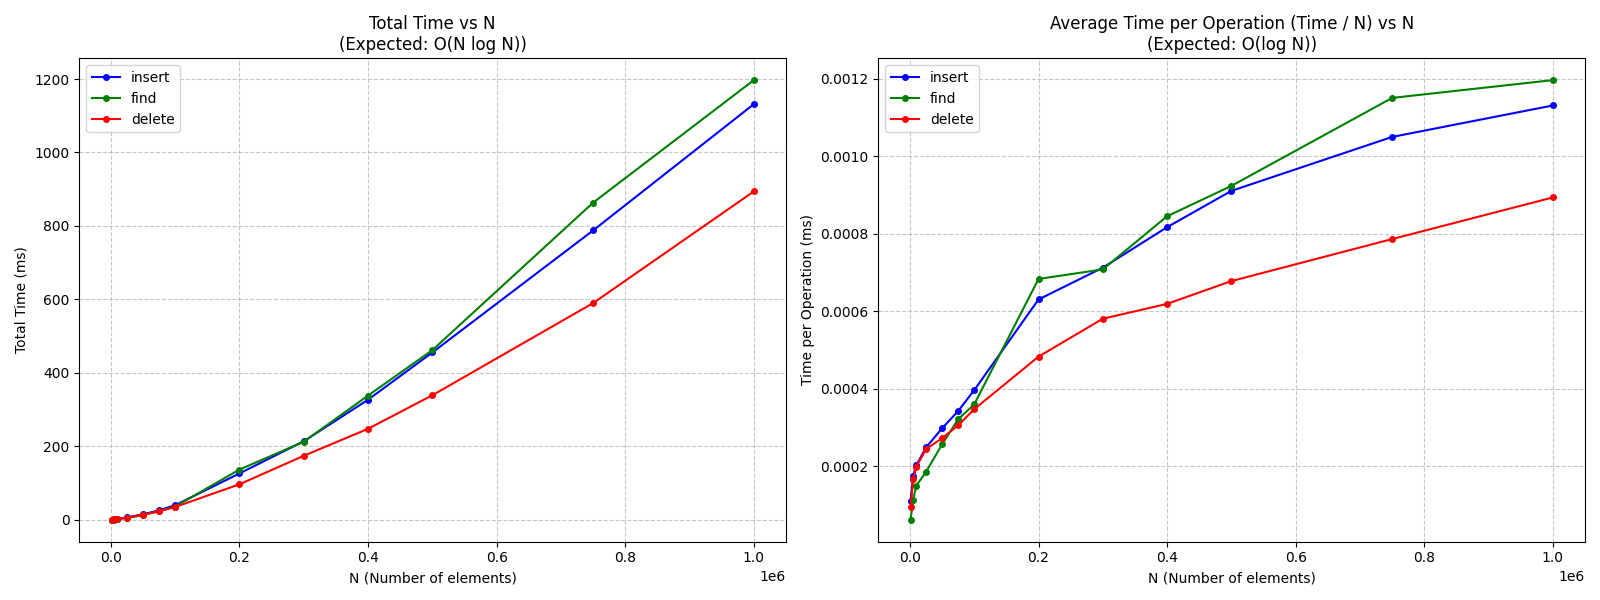
\includegraphics[width=1.0\textwidth]{../results/skip_list_performance.png}
    \caption{Performance of Skip List Operations. Left: Total execution time grows linearly with $N \log N$. Right: Average time per operation grows logarithmically with $N$.}
    \label{fig:perf_plot}
\end{figure}

\subsection{Analysis}
\begin{itemize}
    \item \textbf{Time Complexity Verification:} 
    As shown in the right subplot of Figure \ref{fig:perf_plot}, the average time per operation increases slowly as $N$ grows. The curve fits the logarithmic growth characteristic $O(\log N)$, which aligns with our theoretical analysis. The total time (left subplot) shows a near-linear trend (more precisely $O(N \log N)$ for $N$ operations), confirming the efficiency of the Skip List.
    
    \item \textbf{Operation Comparison:} 
    For smaller $N$ (e.g., $N < 50,000$), the three operations have comparable performance, with \texttt{find} often being slightly faster due to fewer pointer updates compared to \texttt{insert} and \texttt{delete}.
    However, as $N$ increases (e.g., $N > 200,000$), the \texttt{delete} operation becomes significantly faster than \texttt{insert} and \texttt{find}. For instance, at $N=1,000,000$, deletion takes approximately 894 ms, while insertion and search take over 1100 ms. This efficiency in deletion can be attributed to several factors:
    \begin{itemize}
        \item \textbf{Memory Management Overhead:} Insertion requires \texttt{malloc} to allocate new nodes, which is generally more expensive than \texttt{free} used in deletion.
        \item \textbf{Cache Locality:} In our test sequence, deletion is performed immediately after insertion. The nodes to be deleted are likely still in the CPU cache ("hot" data), whereas insertion always allocates new, potentially "cold" memory addresses.
        \item \textbf{Pointer Updates:} Deletion only requires updating the forward pointers of predecessor nodes, whereas insertion requires initializing all forward pointers of the new node plus updating predecessors.
        \item \textbf{Random Number Generation:} Insertion requires generating a random level for each new node, adding computational overhead that deletion avoids.
    \end{itemize}
\end{itemize}

\section{Conclusion}
In this project, we successfully implemented a Skip List data structure in C and conducted a comprehensive performance analysis. Our experimental results confirm that the Skip List provides efficient $O(\log N)$ time complexity for insertion, deletion, and search operations, making it a viable alternative to balanced binary search trees.

\subsection{Future Improvements}
While our implementation is functional and efficient, there are several areas for potential optimization and further study:

\begin{enumerate}
    \item \textbf{Memory Optimization:} Currently, our node structure uses a fixed-size array (\texttt{MAX\_LEVEL}) for forward pointers. This simplifies implementation but wastes memory for nodes with low levels. A dynamic allocation strategy for the forward pointer array could significantly reduce the memory footprint, especially for large $N$.
    
    \item \textbf{Cache-Friendly Layout:} The standard linked-list structure of Skip Lists suffers from poor cache locality compared to B-Trees or arrays. Implementing an "unrolled" Skip List (where each node stores multiple elements) could improve cache performance by reducing pointer chasing.
    
    \item \textbf{Deterministic Skip Lists:} To avoid the worst-case $O(N)$ scenario (though extremely rare), we could explore deterministic variants like the 1-2-3 Skip List, which guarantees strict logarithmic bounds at the cost of slightly more complex insertion/deletion logic.
    
    \item \textbf{Concurrency Support:} Skip Lists are known to be easier to parallelize than balanced trees. Future work could involve implementing a lock-free concurrent Skip List to leverage multi-core processors.
\end{enumerate}

\section{Declaration}
\textit{We hereby declare that all the work done in this project is of our own independent effort.}

\end{document}